\section{Interfaz y control de motores}

El desarrollo de la interfaz entre la PC y los motores del robot se realizó priorizando funcionalidad, simplicidad y robustez. El sistema se diseñó para que la placa controladora actúe únicamente como una unidad de control de bajo nivel, recibiendo comandos desde la PC y ejecutando las órdenes directamente sobre los actuadores, sin necesidad de procesamiento complejo en el microcontrolador.

Este diseño modular permite además implementar distintos modos de operación sin modificar el hardware: control local desde una computadora de abordo, teleoperación remota o integración con sistemas autónomos, cambiando únicamente el medio físico de comunicación.

\subsection{Análisis de Implementación}
El sistema de control está dividido en tres capas software principales:

\begin{itemize}
    \item \textbf{Capa de aplicación (PC):}
Utiliza la clase RobotDriver, que actúa como interfaz de alto nivel (wrapper) para generar comandos de movimiento, torreta y disparo sin interactuar directamente con los frames del protocolo.

    \item \textbf{Capa de comunicación (PC–Microcontrolador):}  
Implementada en la PC en Python mediante RobotConnector, encargada de formar, enviar y validar tramas sobre el enlace UART. Y en el Microcontrolador en C++ mediante RobotListener, encargade de recepción, decodificación y validación de tramas.

    \item \textbf{Capa de control de hardware (Microcontrolador):}
Implementa la clase Robot, encargada del control directo de motores DC, motores paso a paso e IO mediante interrupciones.
\end{itemize}


Dentro de la implementacion las partes mas destacables son la capa de comunicacion y la de control de hardware.

\subsubsection{Comunicacion}

La comunicación entre la PC y la placa se implementó sobre un enlace UART, utilizando un protocolo propio basado en tramas compactas de longitud variable.

\begin{figure}[H]
\centering
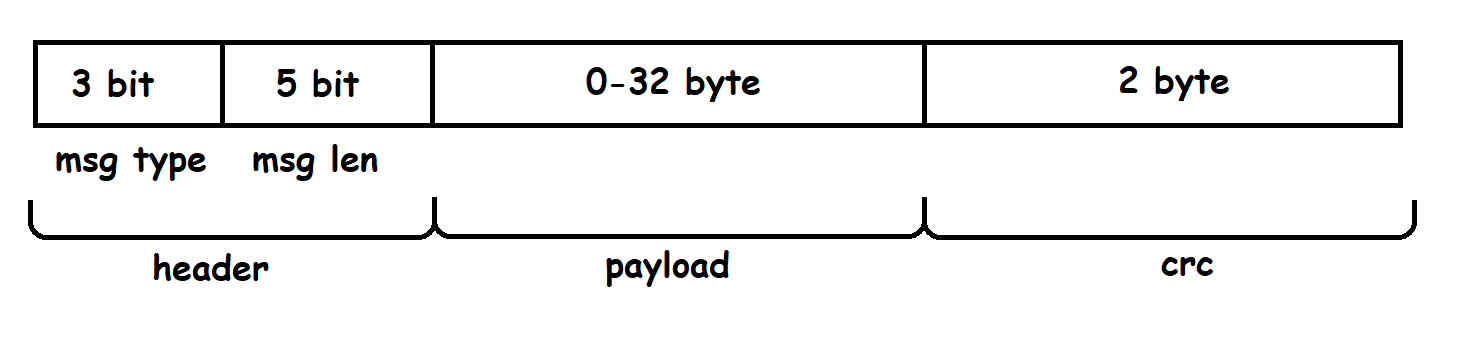
\includegraphics[width=.99\textwidth]{Figures/protocolo.png}
\label{fig:Trama}
\caption{Trama del protocolo}
\end{figure}


\begin{table}[h]
\centering
\begin{tabular}{l l l p{6cm}}
\toprule
\textbf{Tipo} & \textbf{Código} & \textbf{Payload} & \textbf{Uso} \\
\midrule
ping    & 0b000 & No       & Verificación de enlace. \\
data    & 0b001 & Sí       & Envio de data. \\
angle   & 0b010 & No       & Consulta de posición de la torreta. \\
ack     & 0b011 & No       & Confirmación válida. \\
nak     & 0b100 & No       & Error de CRC, solicitar retransmisión. \\
home    & 0b101 & No       & Enviar torreta a origen. \\
metrics & 0b110 & No       & Solicita datos del sistema. \\
stop    & 0b111 & No       & Detener actuadores. \\
\bottomrule
\end{tabular}
\caption{Mensajes, códigos y uso del payload}
\end{table}

El flujo completo de comunicación es el siguiente:

\begin{enumerate}
    \item \textbf{Generación de la trama en la PC:}  
    Se construye la trama, incluyendo el encabezado, el payload y el CRC-16 correspondiente.

    \item \textbf{Transmisión hacia el microcontrolador:}  
    La trama completa se envía.

    \item \textbf{Recepción y decodificación en la placa:}  
    El microcontrolador recibe los bytes, interpreta el encabezado y separa el payload y el CRC recibido.

    \item \textbf{Validación mediante CRC:}  
    La placa calcula localmente el CRC-16 del header y payload recibidos y lo compara con el CRC transmitido:
    \begin{itemize}
        \item Si los valores \textbf{coinciden}, la trama es válida:  
        la placa ejecuta el comando solicitado y responde con una trama de tipo \texttt{ACK}.
        \item Si los valores \textbf{no coinciden}, se considera error de transmisión:  
        la placa responde con una trama \texttt{NAK}.
    \end{itemize}

    \item \textbf{Retransmisión automática en caso de error:}  
    Si la PC recibe un \texttt{NAK}, interpreta que ocurrió un error de comunicación y retransmite automáticamente la última trama enviada, garantizando la entrega confiable del comando.

    \item \textbf{Pedido de datos de telemetria:}  
    Si el controlador recibe un frame de tipo \texttt{metrics}, entonces responde con una trama de tipo \texttt{data} con la información de las métricas, la respuesta de tipo \texttt{data} se interpreta como un \texttt{ACK}.
\end{enumerate}
El CRC utilizado es CRC-16 con polinomio \texttt{0x1021} e inicialización \texttt{0xFFFF}, calculado sobre el header y el payload. 

Ademas se implementa un timeout para la recepción de la confirmación, de esta manera se asegura un funcionamiento robusto del sistema incluso en presencia de ruido o pérdidas temporales en el enlace.


Para controlar el robot se usan principalmente tramas de tipo \texttt{data} compuestas de la siguiente manera:

\texttt{[0b001101][velL, velR, velPitch, velYaw, shoot][CRC]}


Las velocidades estan expresadas entre 0 y 255, siendo 0 velocidad totalmente negativa, 255 maxima velocidad positiva y 128 velocidad 0.

\subsubsection{Drivers}
Para el control del robot se utilizaron dos tipos de actuadores:
\begin{itemize}
    \item Motores DC con puente H, utilizados para tracción.

    \item Motores paso a paso, utilizados para la torreta.
\end{itemize}
Debido a las diferencias entre ambos actuadores, los controladores fueron diseñados de forma independiente.
\subsubsection{Drivers para motor de tracción}
Los puentes H que usan los motores de tracción izquierdo y derecho son controlados mediante tres señales, dos de dirección que controlan el sentido de giro y una de marcha en la que se utiliza PWM benedictino un control de la velocidad de giro de las ruedas.

Para las señales PWM se utilizo el timer0 del microcontrolador.
\subsubsection{Driver motor torreta}
Pese a que los drivers utilizados para los motores stepper de elevación y giro de la torreta son diferentes debido a las diferencias en requisitos de potencia de los motores usados, las señales de control que necesitan son iguales, por lo que a nivel lógico los controladores se pudieron implementar de igual manera.
Ambos drivers requieren una señal digital de dirección y una señal digital cuyo flanco ascendente indica un paso.
Se utilizo el timer1 del microcontrolador para disparar interrupciones, lo que genera un ciclo de control estable para actualizar la señal de control de velocidad y logra un movimiento fluido y controlado de los motores de la torreta.

\subsection{Conclusiones del Análisis de Implementación}

La estructura en tres capas principales que organizan el flujo de información desde la PC hasta los actuadores del robot separa claramente las responsabilidades de alto nivel, comunicación y control físico, lo que simplifica el diseño y facilita la expansión del sistema.

La implementación de un protocolo con confirmación de recepción y validación de tramas brinda robustez al sistema y el uso de los timers internos del micro permitió generar un ciclo de control estable para los actuadores independiente del tiempo de procesamiento de las tramas, lo que permite lograr mayores velocidades angulares en los motores stepper.

Si bien no se implemento la recopilación de datos de telemetria por parte del prototipo, el haberlos contemplado en el protocolo de comunicación hace que en desarrollos futuros sea posible agregar esta funcionalidad sin modificaciones sustanciales de software.



